\section{Introduction}
\label{sec:intro}


Elementary particle physics describes our world in terms of its smallest constituents, fundamental particles, and their interactions. Going from larger to smaller scales, substances around us consist of molecules, molecules consist of atoms, in an atom, there is a nucleus made of neutrons and protons and some number of electrons occupying their orbits around the nucleus. Protons and neutrons have a structure while an electron is not known to have any structure, therefore, an electron is an example of a particle which is considered to be fundamental.\\

Interactions of elementary particles are described by quantum field theories which incorporate principles of the quantum mechanics and the special theory of relativity. The set of such theories, including quantum elecrtrodynamics (QED), quantum chromodynamics (QCD) and the theory of weak interactions is called the Standard Model (SM). It has been proven to be an accurate description of interactions of elementary particles observed by now.\\ 

However, there are several experimental observations which are not described by the SM such as gravity, dark matter, dark energy, matter/antimatter asymmetry and others. Therefore, the SM is not the complete theory of particle interactions. There are several SM extensions offered by theorists as well as radically new theories waiting for the experimental confirmation or disproof. \\

Some SM extensions and new theories predict the existence of heavy particles mass of which possibly lies beyond experimentally reachable energies. The search of these particles is one of the prioritized directions in particle physics. One source of highly energetic elementary particles is cosmic rays. The most energetic particles ever observed came from this source. However, cosmic rays are totally uncontrollable and such highly energetic particles are rare. If we want to produce a large number of particles in a given energy range, we need to use a particle accelerator. A large amount of data allows experimentalists to perform a statistical analysis and increase the probability to find a new particle if it exists.\\

Symmetric colliding beams is the most effective way to produce as heavy particles as possible given the energies of the colliding particles. Comparing to experiments of colliding a single beam to a fixed target, in case of a symmetric collision the total momentum of two colliding particles is zero and, therefore, much larger fraction of energy can transfer to a mass of a new particle.  The Large Hadron Collider (LHC) is such a collider with the highest energy in the world ever built. It can produce the most massive particles to probe physics beyond the SM. It collides two proton ($pp$) beams, two lead ion beams ($Pb-Pb$) or a proton beam to a lead ion beam ($p-Pb$). The design energies for a colliding proton and a colliding lead ion at LHC are~7~TeV and~522~TeV respectively. \\

Compact Muon Solenoid (CMS) is one of two general-purpose detectors at the LHC. It is placed at one of six collision points. CMS has a wide physics program including searches for the beyond SM (BSM) physics as well as the precision measurements of the SM parameters themselves.\\

%In this dissertation the analysis of $pp\rightarrow W\gamma + X$  processes using  leptonic decays of $W\to \ell\nu$ where $\ell = e, \mu$ is reported. The $W\gamma$ productions with leptonic $W$ decays can go through one of the following three processes: initial state radiation where a photon is produced from one of the incoming partons, final state radiation where a photon is radiated off the charged lepton from the $W$ boson decay, and finally when a photon is produced via the triple gauge coupling (TGC) where a photon is emitted from the $W$ boson. \\ 

%To search for the deviations from the SM, one would search for an anomalous TGC which would be indicated by the enhance of the TGC production over the SM prediction. \\

The total and the differential cross section with respect to the photon transverse momentum ($P_T^\gamma$) has been measured. The $P_T^{\gamma}$ is sensitive to the potential anomalous TGC (aTGC) in the high $P_T^{\gamma}$ region. The disagreement between the measured and theoretically predicted differential cross section at the higher $P_T^{\gamma}$ end would be an indication of the possible presence of the aTGC. \\

The rest of this chapter gives general introductory information about the SM while chapter \ref{sec:WgAbout} concentrates on the theory of the SM and BSM $W\gamma$ production and also discusses previous measurements of this process. Chapter \ref{sec:Exp} describes LHC and CMS in more details. Chapter \ref{sec:alignment} explaines on specific aspect of the CMS operation which is the tracker alignment. Finally, chapter \ref{sec:AN_WgMeas} describes the details of the measurement of this dissertation and reports the results.\\ 



%\subsection{Fundamental Particles and Interactions}
\label{sec:Intro_FundParticles}

The SM describes interactions of elementary particles. There are four fundamental interactions: electromagnetic, strong, weak and gravitational. The gravity is not included into the SM but its effect on particles is negligible compared to the other forces which makes it possible to develop a theory of the particle physics and conduct experiments even without having the gravity included into the model.\\ 

All fundamental elementary particles in the SM can be split into three categories by their spins. There are fermions which possess spin s=1/2, there are gauge bosons which are vector particles (s=1) and there is the Higgs boson which is a scalar particle (s=0). \\

The fermions are arranged into three generations, each generation consists of a quark with charge Q=$+$2/3(up, charm, and top quarks), a quark with Q=$-$1/3 (down, strange, and bottom quarks), a charged lepton with Q=$-$1 (electron, muon, and tau-lepton) and a neutrino (electron, muon, and tau neutrinos) which is electrically neutral. Each quark can carry any of three colors: red, blue, or green. Additionally, each fermion has its antiparticle. Therefore, the total number of fundamental fermions is $(6 ($leptons$)+6 ($quarks$) \cdot 3 ($colors$) ) \cdot 2 ($to~include~antiparticles$) = 48$.\\ 

Corresponding particles in different generations have the same charges, spins and interaction properties but masses of particles increase with a generation. These mass differences lead to different decay properties because a particle A can decay to particles B and C only if their masses relate as $m_A > m_B + m_C$. Thus, an electron is a stable particle, a muon decays as $\mu^- \rightarrow e^- + \bar{\nu_e} + \nu_\mu$, a tau-lepton, as the heaviest charged lepton, has the largest number of decay channels amongst the charged leptons: $\tau^- \rightarrow \mu^- + \bar{\nu_\mu} + \nu_\tau$, $\tau^- \rightarrow e^- + \bar{\nu_e} + \nu_\tau$,  $\tau^- \rightarrow \nu_\tau +$ quarks. \\

In addition to fermions, the SM includes gauge bosons which are interaction mediators. They are called mediators because fermions interact with each other by exchanging them. For example, two charged fermions can interact with each other by exchanging a photon. Such interaction is called electromagnetic interaction and a photon is a mediator for the electromagnetic interaction. Similarly, a gluon is a mediator for strong interactions, and W$^{\pm}$ and Z$^0$ bosons are mediators for weak interactions. W$^{\pm}$ and Z$^0$ bosons are massive while a photon and a gluon are massless particles. \\

The last SM particle is the Higgs boson. The Higgs boson is a scalar neutral particle which is playing a critical role in the electroweak symmetry breaking. The Higgs mechanism explains how $W$ and $Z$ bosons become massive particles.\\

All the particles are summarized in Fig.~\ref{fig:SMtable}. These and only these fundamental particles and their antiparticles have been discovered by now. However, there are many composite particles which are called hadrons. Hadrons can consist of three quarks (baryons), quark and antiquark (meson), or three antiquarks (antibaryons). Hadrons always possess an integer charge.\\

Most of the particles are short-lived and decay within microseconds. The only stable particles are protons and antiprotons, electrons and positrons, neutrinos and antineutrinos, photons, and, in some sense, gluons. However, if a particle cannot decay, it does not mean that it would live forever. There are many different kinds of reactions in which particles can disappear. Antiprotons and positrons would immediately annihilate with protons and electrons, photons can be absorbed by charged particles, electrons and protons can scatter to produce neutrons and neutrinos and many other reactions are possible.\\ 

In this dissertation, the study of $pp\rightarrow W\gamma + X$ process where the $W$ decays as $W\to \ell\nu$ where $\ell = e, \mu$ is reported. The $W\gamma$ production with leptonic $W$ decays proceeds through one of the following three processes: the initial state radiation where a photon is emitted from one of the incoming partons, the final state radiation where a photon is radiated off the charged lepton from the $W$ boson decay, and, finally, the triple gauge coupling (TGC) where a photon is emitted from the $W$ boson. Many BSM theories predict an enchancement of the TGC production over the SM value and, therefore, the experimental search for such an enchancement is a good test for such theories.\\ 
%The total and the differential cross section with respect to the photon transverse momentum ($P_T^\gamma$) has been measured. The $P_T^{\gamma}$ is sensitive to the potential anomalous TGC (aTGC) in the high $P_T^{\gamma}$ region. The disagreement between the measured and theoretically predicted differential cross section at the higher $P_T^{\gamma}$ end would be an indication of the possible presence of the aTGC.

%In this dissertation a process is studied where quark and antiquark interact to produce a $W$ boson which then decay as $W^\pm \rightarrow e^\pm \nu_e(\bar{\nu_e})$ or $W^\pm \rightarrow \mu^\pm \nu_\mu(\bar{\nu_\mu}) $. A photon is radiated off a quark or antiquark, a charged lepton or a $W$ boson. The most interesting mechanism out of three is a radiation from a $W$ boson because this is the triple gauge coupling where we potentially can have a new physics. 

Therefore, the focus of this study is an interaction between a photon and a $W$ boson however many other SM particles are relevant too. Thus, a charged lepton and a neutrino appear as the final state particles, a quark and an antiquark appear as initial state particles and all fundamental particles except the Higgs boson participate in various background processes. Subsections \ref{sec:Intro_Electroweak}-\ref{sec:Intro_ppCollisions}, chapter \ref{sec:WgAbout} and \cite{ref_Griffiths} describe particle interactions in more details.\\


\begin{figure}[htb]
  \begin{center}
    {\includegraphics[width=0.90\textwidth]{../figs/Intro/StandardModel.png}}
    \caption{Standard Model Particles and Interations. Source of the figure: \cite{ref_fig_SM}.}
    \label{fig:SMtable}
  \end{center}
\end{figure}






%\subsection{Electroweak Interactions}
\label{sec:Intro_Electroweak}



% The style needs to be improved. Some places contain very chopped language.
% Consider this passage, way too “chopped”:
% > Elementary processes with W and Z bosons are shown in Fig. 3. An electric charge must be
% > conserved at any vertex. Therefore, if a charged lepton enters and radiates a W boson, a
% > neutrino or antineutrino escapes (top left in Fig. 3). That is how a W boson interacts with a
% > charged lepton and a neutrino. A lepton flavor number is always conserved in this interaction (Tab. 1).
%Consider using math mode for single character particle names, such as $c$ or $d$, to make them distinct in the text.

All electrically charged particles participate in electromagnetic interactions. Photon, the mediator of the electromagnetic interactions, is a spin-one electrically neutral massless particle. All electromagnetic interactions can be reduced to one elementary process (Fig. \ref{fig:feynmEM}, left). This process reads: an electron enters, radiates or absorbs a photon, and escapes. Although there is an electron is drawn in this figure, it can be any other charged particle as well. Such elementary process itself is forbidden by the energy conservation law but this element is a base of actual process (for example, Fig. \ref{fig:feynmEM}, middle and right). Such graphical representations of the particle physics processes are called Feynman diagrams.\\ 

\begin{figure}[htb]
  \begin{center}
    {
\includegraphics[width=0.90\textwidth]{../figs/Intro/feynmEM.png}}
    \caption{Electromagnetic interations}
    \label{fig:feynmEM}
  \end{center}
\end{figure}

\begin{figure}[htb]
  \begin{center}
    {
\includegraphics[width=0.90\textwidth]{../figs/Intro/feynmW.png}}
    \caption{Weak interations}
    \label{fig:feynmW}
  \end{center}
\end{figure}


As for the weak interactions, there are two kinds of them: neutral (mediated by a Z boson) and charged (mediated by a W$\pm$ boson). Elementary processes with W and Z bosons are shown in Fig. \ref{fig:feynmW}. Because the electric charge must be conserved at any vertex, a particle radiating or absorbing a W boson converts to a different particle. Thus, a charged lepton converts to a neutrino (or vice versa) as shown in Fig. \ref{fig:feynmW}, top left. A lepton flavor number is always conserved in such interactions (lepton flavor numbers assigned to different lepton are summarized in Tab. \ref{tab:LeptonFlavorNumber}), thus an electron always converts to an electron neutrino, a muon always converts to a muon neutrino etc.\\

 \begin{table}[h]
  \begin{center}
  \caption{ Lepton Flavor Number}
  \begin{tabular}{|c|c|c|c|}
     particles & $L_e$ & $L_{\mu}$ & $L_{\tau}$ \\ \hline
     $e^-,\nu_e$ &  +1  &  0  &  0  \\ \hline 
     $e^+, \bar{\nu_e}$ &  -1  &  0  &  0  \\ \hline 
     $\mu^-,\nu_{\mu}$ &  0  &  +1  &  0  \\ \hline 
     $\mu^+, \bar{\nu_{\mu}}$ &  0  &  -1  &  0  \\ \hline 
     $\tau^-,\nu_{\tau}$ &  0  &  0  &  +1  \\ \hline 
     $\tau^+, \bar{\nu_{\tau}}$ &  0  &  0  &  -1  \\ \hline 
  \end{tabular}
  \label{tab:LeptonFlavorNumber}
  \end{center}
 \end{table}

From top middle diagram in Fig. \ref{fig:feynmW} we see that if a quark with Q=-1/3 enters, then a quark with Q=+2/3 escapes and, therefore, the flavor of the quark has changed. The charged weak interaction is the only interaction which changes a quark flavor. The probability of each of three quarks with Q=+2/3 to be born is determined by the Cabibbo–Kobayashi–Maskawa matrix and is the highest for the quark of the same generation as an initial state quark (in this particular case, $d$ is the initial state quark and $u$ has the highest probability to be produced after an interaction with a W boson but $c$ and $t$ can also be produced if there is enough energy).\\

An elementary process of a neutral weak interactions is an emission of a Z boson off a fermion line (right top diagram in Fig. \ref{fig:feynmW}). An electron is shown here as an example however it also could be any lepton, antilepton, quark or antiquark. Diagrams with a Z boson are very similar to ones with a photon except a photon can only be radiated off a charged particle but a Z boson can also be radiated off a neutrino or antineutrino.\\

The bottom diagrams in Fig. \ref{fig:feynmW} are gauge coupling diagrams. Gauge couplings include self-coupling of a W boson, its interaction with Z boson and its electromagnetic radiation of a photon. WWZ, WW$\gamma$, WWZZ, WWZ$\gamma$, WW$\gamma\gamma$ and WWWW vertices are all possible in the SM.\\

Electromagnetic and weak interactions are unified by the electroweak theory. This theory considers these two forces as different manifestations of the electroweak force. While both forces can be described by very similar formalism, there is also a big difference between them: weak interactions are mediated by heavy bosons ($M_W=80$ GeV, $M_Z=91$ GeV) while electromagnetic interactions are described by a massless photon. \\

To explain this phenomenon, the Higgs mechanism was introduced. The mechanism predicted an existence of an additional boson - the Higgs boson. The Higgs boson was a missing piece of the SM for many years and was finally discovered in 2012 at the LHC by ATLAS and CMS collaborations through the processes shown in Fig.\ref{fig:higgsProduction}.\\ 

\begin{figure}[htb]
  \begin{center}
    {\includegraphics[width=0.95\textwidth]{../figs/Intro/FeynmanHiggs.png}}
    \caption{Higgs production and decay}
    \label{fig:higgsProduction}
  \end{center}
\end{figure}

The measurement in this dissertation is an electroweak measurement because the process involves a W boson. It includes an interaction of a W boson with leptons and quarks as well as the gauge coupling WW$\gamma$. Thus, the measurement is a good test of the SM electroweak theory.\\ 




%\subsection{The Higgs Boson}
\label{Intro_Higgs}

% BAD SECTION
% NEEDS TO BE SIGNIFICANTLY REWORKED

\begin{figure}[htb]
  \begin{center}
    {\includegraphics[width=0.95\textwidth]{../figs/Intro/FeynmanHiggs.png}}
    \caption{Higgs production and decay}
    \label{fig:higgsProduction}
  \end{center}
\end{figure}

%  I feel that there is a number of imprecise statements here that need to be corrected. Here are examples.
%   (A side note: quant is not what you mean, check the dictionary. You want to say “quantum”)
%   I would not say that the Higgs boson is a quantum of the Higgs field. The Higgs field is a doublet of complex fields, i.e. it has four components. According to wikipedia wording, for example, “it is a quantum excitation of one of the four components of the Higgs field. "
% This part: "discovered by ATLAS and CMS collaborations in the reaction shown in Fig. 4 in γγ and ZZ decay channels”
% The diagram in Fig. 4 is not appropriate for ZZ.
% "the same approach can be used to introduced masses of all elementary particles.” - but what about neutrinos? I am not sure if our favorite explanation of neutrino masses is the Higgs.
% It is not intuitive to me that larger mass means stronger interaction with the Higgs field,
% I am not sure why you say that.
% "that is how is gets its inertia”: consider rephrasing.









%\subsection{Strong Interactions}
\label{sec:Intro_QCD}

\begin{figure}[htb]
  \begin{center}
    {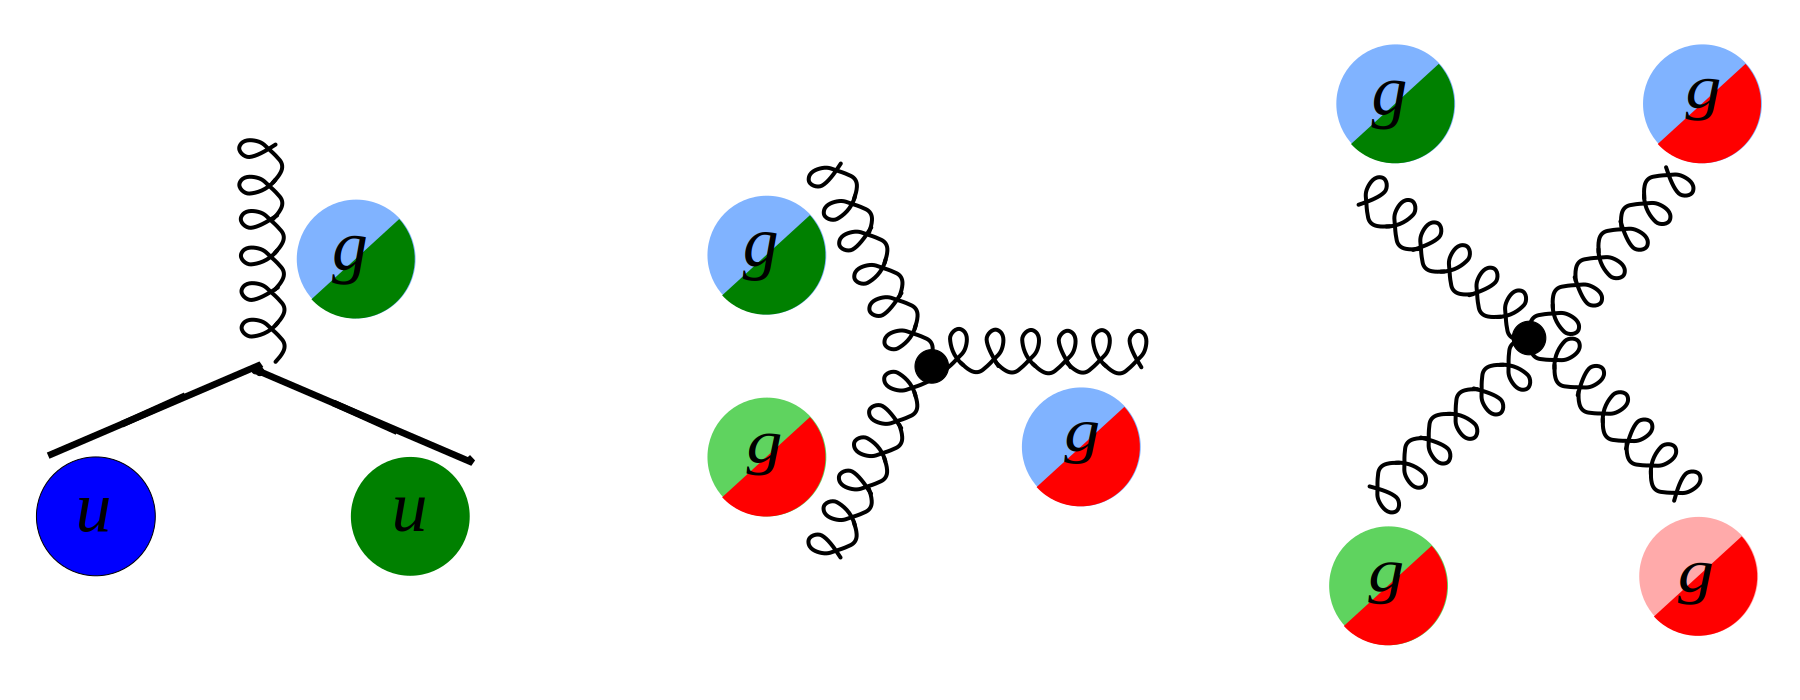
\includegraphics[width=0.90\textwidth]{../figs/Intro/feynmStrong.png}}
    \caption{Strong interations}
    \label{fig:feynmStrong}
  \end{center}
\end{figure}

 %  Again, I do not see a connective narrative. Paragraphs are sets of loosely connected sentences, the section is a set of loosely connected paragraphs. Needs imporvement.
% Somewhat reverse flow of ideas, example:
% > There are eight types of gluons corresponding to different color-anticolor combinations.
% > Gluons are spin-one massless electrically neutral particles.
% First, you should say what gluons ARE, and then you can say what types of gluons exist.
% > Gluons possess color charges, therefore, they can self-interact.
% The emphasis of this statement is that gluons possess color charges, which is odd because you already mentioned it some number of times above (which adds to the feeling of reverse flow).
% Instead, the emphasis of the sentence should be that they can self-inteact.
% Some incorrect information, for example:
% "it becomes larger as the distance becomes smaller” about the coupling constant: it becomes smaller at smaller distances, larger at larger distances.

The third fundamental force after the electromagnetic and weak ones is the strong force. The strong force is responsible for glueing protons and neutrons together in the nuclea as well as for forming protons and neutrons themselves. The strong interactions are performed by exchanging gluons which are spin-one massless electrically neutral particles.  \\

The elementary strong processes are shown in Fig. \ref{fig:feynmStrong}. There are three elementary processes: qqg, ggg and gggg, all are involving particles with color charges. Thus, gluons couple to quarks and self-couple. Color charges must be conserved at each elementary process of the strong interaction. And because quarks can possess three colors, there are eight types of gluons to cover all possible color exchanges. \\

The coupling constant of the strong interaction depends on a distance between interacting particles: it becomes larger as the distance becomes larger. This property leads to two consequences specific to the strong force: the confinement and the asymptotic freedom.\\

The confinement is the property of quarks to always stay in the colorly neutral combinations (hadrons), it forbids the existence of free quarks. A combination becomes colorly neutral when there is the same amount of color and anticolor or if there is the same amount of each of the three colors.  There are two types of hadros: mesons (comprised of a quark and antiquarks with the opposite color charges) and baryons (comprised of three quarks: a red, a green and a blue one). The widely known particles a proton and a neutron are baryons.\\

The asymptotic freedom means that when quarks are very close to each other they almost do not interact with each other and therefore they are free. When the distance between quarks is low which corresponds to high energy, and thus the coupling constant $1/\alpha_s \ll 1$ is low, the strong interactions can be described by a perturbative quantum field theory which is called quantum chromodynamics (QCD).\\

The W$\gamma$ process being measured in this dissertation is not intended to test QCD, but a good understanding of QCD is essential for performing this measurement. First of all, QCD describes the dynamics of quarks and gluons within colliding protons and predicts probabilities of one or another quark-antiquark pair to annihilate. Secondly, the QCD corrections to the Feynman diagrams of the process are large and has to be taken into account in producing simulation. Possible QCD correction include quark-gluon loops at any of three quark lines as well as exchanges of gluons between different quark lines.\\
 

%\subsection{Physcis of Proton-Proton Collisions}
Physcis of Proton-Proton Collisions

%\section{Open Questions of the Standard Model}


While the SM is an accurate description of all particle physics experimental results, there are certain phenomena which are not included into the SM. In this subsection we discuss some of them.

The gravitational interactions do not fit into the SM. It is the open question whether the quantum theory of gravity is possible and whether there is a mediator of the gravitational interactions. Also, it is not known why the gravitational force is so much weaker than the other forces. One possible explanation comes from a theory which predicts extra spatial dimensions beyond the three we experience (e.g. the string theory). In this case, it is possible that the gravitational force is shared with other dimensions and only a fraction is available in our three dimensions.

Another mystery of the universe is its composition: it is known from the studies of the gravitational effects that our universe consists of dark energy by 68\%, of dark matter by 27\% and of baryon matter only by 5\%~\cite{ref_NASA}. The dark energy resists the gravitational attraction and accelerates the expansion of the universe, and is not detectable by any effects except gravitational. The understanding of dark energy is a question of general relativity rather than particle physics. The dark matter, however, likely consists of particles and therefore is a subject of particle physics. It does not radiate and that is why it cannot be detected by telescopes. The nature of the dark matter is not known but its constituents must be very stable to remain since the Big Bang. The theory of the supersymmetry which is unifying fundamental particles and mediators predicts many of new heavy particles and the lightest supersymmetric particle, the neutralino, is a good candidate for dark matter.

One more open question is the reason for the matter/antimatter asymmetry. Matter and antimatter should have been created in the same amount at the moment of the Big Bang. Most of it has annihilated but because of asymmetry, there was more matter than antimatter which led to the state of the Universe we observe now. There is a phenomenon of the CP-violation in weak interactions observed and described which predicts the asymmetry at a certain level. However, the effect of the CP-violation is not large enough to account for the observed amount of the matter and, therefore, the total matter/antimatter asymmetry remains unexplained. 

The measurement of the $W\gamma$ production in $pp$ collisions has a goal to both test the SM and search for the BSM physics. We measure a cross section differential in the component of the photon momentum, transverse to the beamline (referred as photon transverse momentum, or $P_T^{\gamma}$). The low $P_T^{\gamma}$ region is not expected to be affected by any new physics and must agree well with the SM predictions while the high $P_T^{\gamma}$ region may indicate an existence of new physics if there is an enhancement over the SM predictions. The excess would be indirect evidence of the BSM particles like supersymmetric particles or additional gauge bosons which could be part of the explanation of the dark matter presence or difference in magnitudes of different interactions. More theoretical details about the SM description of W$\gamma$ process as well as possible BSM physics are given in Ch.~\ref{sec:WgAbout}.    

%Grand unification and super unification


